\documentclass[10pt]{article}

\usepackage[T1]{fontenc}
\usepackage[left=2cm, right=2cm, top=2cm, bottom=2cm]{geometry}
\usepackage[skins]{tcolorbox}
\usepackage{hyperref, fancyhdr, lastpage, tocloft, ragged2e, multicol}
\usepackage{amsmath, amssymb, amsthm}
\usepackage{tkz-tab}

\def\pagetitle{Fonctions usuelles}

\title{\bf{\pagetitle}\\\large{Corrigé}}
\date{Septembre 2023}
\author{DARVOUX Théo}

\DeclareMathOperator{\ch}{ch}
\DeclareMathOperator{\sh}{sh}
\DeclareMathOperator{\tah}{th}

\hypersetup{
    colorlinks=true,
    citecolor=black,
    linktoc=all,
    linkcolor=blue
}

\pagestyle{fancy}
\cfoot{\thepage\ sur \pageref*{LastPage}}


\begin{document}
\renewcommand*\contentsname{Exercices.}
\renewcommand*{\cftsecleader}{\cftdotfill{\cftdotsep}}
\maketitle
\hrule
\tableofcontents
\vspace{0.5cm}
\hrule

\thispagestyle{fancy}
\fancyhead[L]{MP2I Paul Valéry}
\fancyhead[C]{\pagetitle}
\fancyhead[R]{2023-2024}
\allowdisplaybreaks

\addcontentsline{toc}{section}{Exponentielle and friends.}

\section*{Exercice 3.1 [$\blacklozenge\lozenge\lozenge$]}
\begin{tcolorbox}[enhanced, width=6in, center, size=fbox, fontupper=\large, drop shadow southwest]
    Résoudre $2\ln\left(\frac{x+3}{2}\right)=\ln(x)+\ln(3)$, sur $\mathbb{R}^*_+$.\\
    Soit $x\in\mathbb{R^*_+}$.\\
    On a :
    \begin{align*}
        &2\ln\left(\frac{x+3}{2}\right)=\ln(x)+\ln(3)\\
        \iff&\ln\left(\left(\frac{x+3}{2}\right)^2\right)=\ln(3x)\\
        \iff&\frac{(x+3)^2}{4}=3x\\
        \iff&x^2-6x+9=0\\
        \iff&x=3
    \end{align*}
    Ainsi, $3$ est l'unique solution.
\end{tcolorbox}
\addcontentsline{toc}{section}{\protect\numberline{}Exercice 3.1}

\section*{Exercice 3.2 [$\blacklozenge\blacklozenge\lozenge$]}
\begin{tcolorbox}[enhanced, width=6in, center, size=fbox, fontupper=\large, drop shadow southwest]
    Résoudre l'équation $ch(x)=2$. Que dire des solutions ?\\
    Soit $x\in\mathbb{R}$.\\
    On a :
    \begin{align*}
        &\frac{e^x+e^{-x}}{2}=2\\
        \iff&e^x+e^{-x}=4\\
        \iff&e^{2x}-4e^x+1=0\\
        \iff&e^x=2\pm\sqrt{3}\\
        \iff&x=\ln(2\pm\sqrt{3})
    \end{align*}
    Ainsi, $\ln(2-\sqrt{3})$ et $\ln(2+\sqrt{3})$ sont les uniques solutions dans $\mathbb{R}$.\\
    On remarque que :
    \begin{align*}
        \ln(2+\sqrt{3})=-\ln\left(\frac{1}{2+\sqrt{3}}\right)=-\ln\left(2-\sqrt{3}\right)
    \end{align*}
    Les solutions sont opposées.
\end{tcolorbox}
\addcontentsline{toc}{section}{\protect\numberline{}Exercice 3.2}

\section*{Exercice 3.3 [$\blacklozenge\lozenge\lozenge$]}
\begin{tcolorbox}[enhanced, width=6in, center, size=fbox, fontupper=\large, drop shadow southwest]
    Résoudre sur $\mathbb{R}^*_+$ l'équation $x^{\sqrt{x}}=\sqrt{x}^x$.\\
    Soit $x\in\mathbb{R}^*_+$.\\
    On a :
    \begin{align*}
        &x^{\sqrt{x}}=\sqrt{x}^x\\
        \iff&e^{\sqrt{x}\ln{x}}=e^{x\ln(\sqrt{x})}\\
        \iff&\sqrt{x}\ln(x)=\frac{x}{2}\ln(x)\\
        \iff&\ln(x)(\sqrt{x}-\frac{x}{2})=0\\
        \iff&\ln(x)=0\text{ ou } \sqrt{x}=\frac{x}{2}\\
        \iff&x=1\text{ ou }\sqrt{x}=2\\
        \iff&x=1\text{ ou }x=4
    \end{align*}
    Les uniques solutions sont donc $1$ et $4$.
\end{tcolorbox}
\addcontentsline{toc}{section}{\protect\numberline{}Exercice 3.3}

\section*{Exercice 3.4 [$\blacklozenge\lozenge\lozenge$] Trigonométrie hyperbolique.}
\begin{tcolorbox}[enhanced, width=7in, center, size=fbox, fontupper=\large, drop shadow southwest]
    1. Montrer que pour tous réels $a$ et $b$, on a
    \begin{itemize}
        \item[(a)] $\ch(a+b)=\ch(a)\ch(b)+\sh(a)\sh(b)$.
        \item[(b)] $\sh(a+b)=\sh(a)\ch(b)+\ch(a)\sh(b)$.
        \item[(c)] Trouver une identité pour $\tah(a+b)$.
    \end{itemize}
    2. Pour $x$ réel, on pose $t=\tah\left(\frac{x}{2}\right)$. Montrer que
    \begin{equation*}
        \text{(a) } \ch(x)=\frac{1+t^2}{1-t^2} \hspace{0.5cm} \text{(b) } \sh(x)=\frac{2t}{1-t^2} \hspace{0.5cm} \text{(c) } \tah{x}=\frac{2t}{1+t^2}
    \end{equation*}
    1.\\
    (a)
    \begin{align*}
        \ch(a)\ch(b)+\sh(a)\sh(b)&=\frac{e^{a+b}+e^{-a-b}}{2}=\ch(a+b)
    \end{align*}
    (b)
    \begin{align*}
        \sh(a)\ch(b)+\ch(a)\sh(b)&=\frac{e^{a+b}-e^{a-b}}{2}=\sh(a+b)
    \end{align*}
    (c)
    \begin{align*}
        \tah(a+b)&=\frac{\sh(a)\ch(b)+\ch(a)\sh(b)}{\ch(a)\ch(b)+\sh(a)\sh(b)}\\
    \end{align*}
    On divise en haut et en bas par $\ch(a)\ch(b)$.
    \begin{align*}
        \tah(a+b)&=\frac{\frac{\sh(a)}{\ch(a)}+\frac{\sh(b)}{\ch(b)}}{1+\frac{\sh(a)}{\ch(a)}\cdot\frac{\sh(b)}{\ch(b)}}=\frac{\tah(a)+\tah(b)}{1+\tah(a)\tah(b)}
    \end{align*}
\end{tcolorbox}

\begin{tcolorbox}[enhanced, width=7in, center, size=fbox, fontupper=\large, drop shadow southwest]
    2.\\
    (a)
    \begin{align*}
        \frac{1+t^2}{1-t^2}&=\frac{1+\tah^2(\frac{x}{2})}{1-\tah^2(\frac{x}{2})}=\frac{\ch^2(\frac{x}{2})+\sh^2(\frac{x}{2})}{\ch^2(\frac{x}{2})-\sh^2(\frac{x}{2})}\\
        &=\ch^2\left(\frac{x}{2}+\frac{x}{2}\right)=\ch(x)
    \end{align*}
    (b)
    \begin{align*}
        \frac{2t}{1-t^2}&=\frac{2\tah(\frac{x}{2})}{1-\tah^2(\frac{x}{2})}=\frac{2\sh(\frac{x}{2})\ch(\frac{x}{2})}{\ch^2(\frac{x}{2})-\sh^2(\frac{x}{2})}\\
        &=\sh\left(\frac{x}{2}+\frac{x}{2}\right)=\sh(x)
    \end{align*}
    (c)
    \begin{align*}
        \frac{2t}{1+t^2}&=\frac{2\tah(\frac{x}{2})}{1+\tah^2(\frac{x}{2})}=\frac{2\sh(\frac{x}{2})\ch(\frac{x}{2})}{\ch^2(\frac{x}{2})+\sh^2(\frac{x}{2})}\\
        &=\frac{\sh(x)}{\ch(x)}=\tah(x)
    \end{align*}
    \qed
\end{tcolorbox}
\addcontentsline{toc}{section}{\protect\numberline{}Exercice 3.4}

\section*{Exercice 3.5 [$\blacklozenge\blacklozenge\lozenge$]}
\begin{tcolorbox}[enhanced, width=6in, center, size=fbox, fontupper=\large, drop shadow southwest]
    Sans calculatrice, comparer $\pi^e$ et $e^\pi$.\\
    Soit $f:x\mapsto\frac{x}{\ln(x)}$. $f$ est dérivable sur $\mathbb{R}^*_+$, de dérivée :
    \begin{equation*}
        f':\begin{cases}\mathbb{R}^*_+\rightarrow\mathbb{R}\\x\mapsto\frac{\ln(x)-1}{\ln^2(x)}\end{cases}
    \end{equation*}
    Un magnifique tableau de variations :
    \begin{center}
        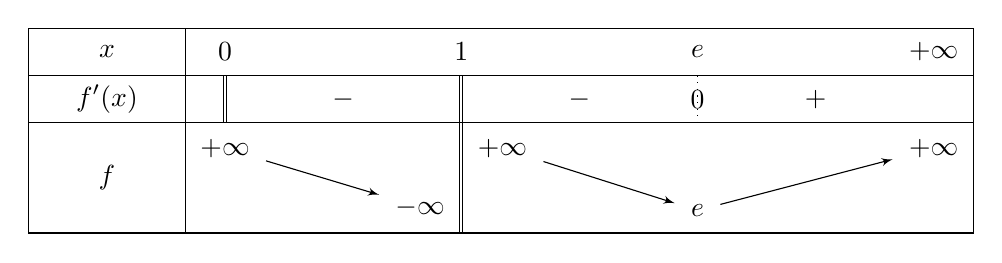
\begin{tikzpicture}
            \tkzTabInit[espcl=3]{$x$/0.6,$f'(x)$/0.6,$f$/1.4}
            {$0$,$1$,$e$,$+\infty$}
            \tkzTabLine{d,-,d,-,z,+}
            \tkzTabVar{+/$+\infty$,-D+/$-\infty$/$+\infty$,-/$e$,+/$+\infty$}
        \end{tikzpicture}
    \end{center}
    On en conclut que :
    \begin{align*}
        &\frac{\pi}{\ln(\pi)}>e\\
        \iff&\pi>e\ln(\pi)\\
        \iff&e^\pi>e^{e\ln{\pi}}\\
        \iff&e^\pi>\pi^e
    \end{align*}
    Donc $e^\pi>\pi^e$.
\end{tcolorbox}

\addcontentsline{toc}{section}{\protect\numberline{}Exercice 3.5}

\section*{Exercice 3.6 [$\blacklozenge\blacklozenge\blacklozenge$]}
\begin{tcolorbox}[enhanced, width=6in, center, size=fbox, fontupper=\large, drop shadow southwest]
    1. Étudier les variations de $f:x\mapsto\sqrt[3]{x}-\sqrt[3]{x+1}$.\\
    2. Des deux nombres $\sqrt[3]{2}+\sqrt[3]{4}$ et $\sqrt[3]{24}$, lequel est le plus grand ?\\[0.5cm]
    1. $f$ est définie, continue et dérivable sur $\mathbb{R}_+$ de dérivée :
    \begin{equation*}
        f':\begin{cases}\mathbb{R}_+\rightarrow\mathbb{R}\\x\mapsto \frac{1}{3}\left(\frac{1}{x^{2/3}}-\frac{1}{(x+1)^{2/3}}\right)\end{cases}
    \end{equation*}
    On a :
    \begin{center}
        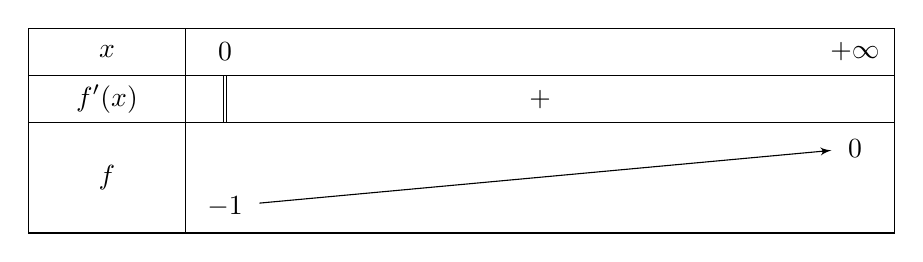
\begin{tikzpicture}
            \tkzTabInit[espcl=8]{$x$/0.6,$f'(x)$/0.6,$f$/1.4}
            {$0$,$+\infty$}
            \tkzTabLine{d,+,}
            \tkzTabVar{-/$-1$,+/$0$}
        \end{tikzpicture}
    \end{center}
    2. 
    \begin{align*}
        &\sqrt[3]{2}+\sqrt[3]{4}-\sqrt[3]{24}\\
        =&\sqrt[3]{2}+\sqrt[3]{4}-2\sqrt[3]{3}\\
        =&(\sqrt[3]{2}-\sqrt[3]{3})-(\sqrt[3]{3}-\sqrt[3]{4})
    \end{align*}
    Or $f$ est croissante sur $\mathbb{R}_+$, ainsi : $\sqrt[3]{3}-\sqrt[3]{4}>\sqrt[3]{2}-\sqrt[3]{3}$.\\
    On en conclut que $\sqrt[3]{24}>\sqrt[3]{2}+\sqrt[3]{4} $.
\end{tcolorbox}

\addcontentsline{toc}{section}{\protect\numberline{}Exercice 3.6}

\section*{Exercice 3.7 [$\blacklozenge\blacklozenge\lozenge$]}
\begin{tcolorbox}[enhanced, width=6in, center, size=fbox, fontupper=\large, drop shadow southwest]
    1. Soit $\alpha$ un réel et $x>-1$. Comparer $(1+x)^\alpha$ et $1+\alpha x$ (on discutera selon les valeurs de $\alpha$).\\
    2. Soit $\alpha\in[0,1]$ et $n\in\mathbb{N}^*$. Montrer que
    \begin{equation*}
        \prod_{k=1}^n{\left(1+\frac{\alpha}{k}\right)}\geq(n+1)^\alpha
    \end{equation*}
    1. Posons $f:x\mapsto(1+x)^\alpha-1-\alpha x$. $f$ est définie, continue et dérivable sur $]-1,+\infty[$ de dérivée :
    \begin{equation*}
        g:\begin{cases}]-1,+\infty[\rightarrow\mathbb{R}\\x\mapsto\alpha((1+x)^{\alpha-1}-1)\end{cases}
    \end{equation*}
    Alors :\\
    $\circledcirc$ Si $\alpha\in]0,1[$:
    \begin{center}
        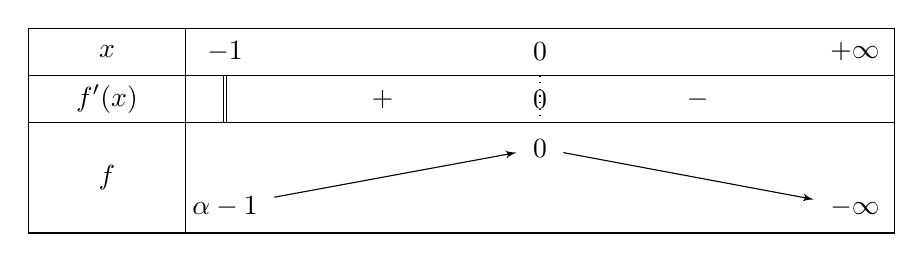
\begin{tikzpicture}
            \tkzTabInit[espcl=4]{$x$/0.6,$f'(x)$/0.6,$f$/1.4}
            {$-1$,$0$,$+\infty$}
            \tkzTabLine{d,+,z,-,}
            \tkzTabVar{-/$\alpha-1$,+/$0$,-/$-\infty$}
        \end{tikzpicture}
    \end{center}
    $\circledcirc$ Si $\alpha\in]1,+\infty[$:
    \begin{center}
        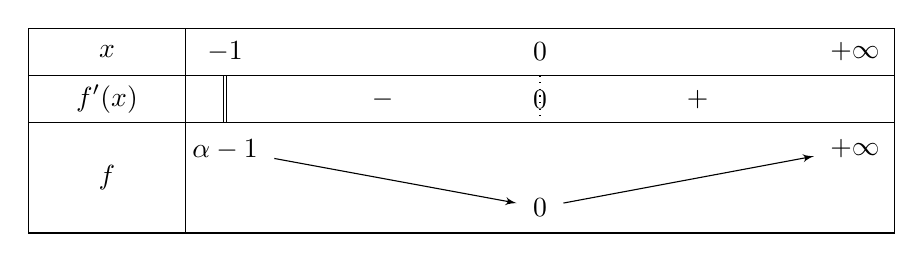
\begin{tikzpicture}
            \tkzTabInit[espcl=4]{$x$/0.6,$f'(x)$/0.6,$f$/1.4}
            {$-1$,$0$,$+\infty$}
            \tkzTabLine{d,-,z,+,}
            \tkzTabVar{+/$\alpha-1$,-/$0$,+/$+\infty$}
        \end{tikzpicture}
    \end{center}
    $\circledcirc$ Si $\alpha\in]-\infty,0[$:
    \begin{center}
        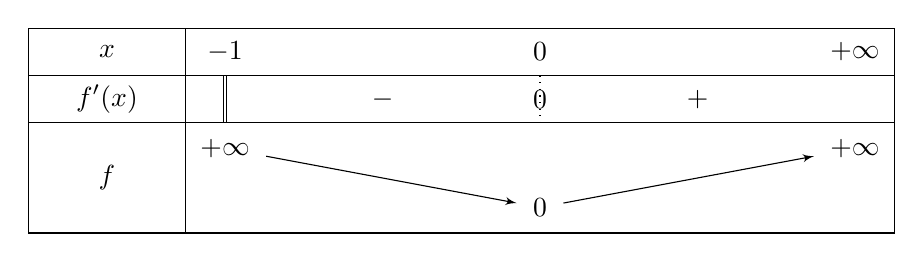
\begin{tikzpicture}
            \tkzTabInit[espcl=4]{$x$/0.6,$f'(x)$/0.6,$f$/1.4}
            {$-1$,$0$,$+\infty$}
            \tkzTabLine{d,-,z,+,}
            \tkzTabVar{+/$+\infty$,-/$0$,+/$+\infty$}
        \end{tikzpicture}
    \end{center}
    Ainsi, $(1+x)^\alpha > 1+\alpha x$ lorsque $\alpha\notin[0,1]$.
\end{tcolorbox}

\begin{tcolorbox}[enhanced, width=6in, center, size=fbox, fontupper=\large, drop shadow southwest]
    2. D'après l'inégalité précédente, on a :
    \begin{align*}
        \prod^n_{k=1}{\left(1+\frac{\alpha}{k}\right)}\geq\prod^n_{k=1}{\left(1+\frac{1}{k}\right)^\alpha}=\prod^n_{k=1}{\frac{(k+1)^\alpha}{k^\alpha}}=(n+1)^\alpha
    \end{align*}
    \qed
\end{tcolorbox}

\addcontentsline{toc}{section}{\protect\numberline{}Exercice 3.7}

\end{document}